
\RequirePackage{etex}

% Vi benytter 2 sidet, a4 størrelse og dansk sprog. 
\documentclass[11pt,a4paper,twoside,danish]{memoir}


\usepackage[paper=A4,pagesize]{typearea}
   
\usepackage[utf8]{inputenc} % danske tegn
\usepackage[danish]{babel} % dansk sprogpakke

% Hvis engelsk sprog ønskes, uncomment denne
% \usepackage[english]{babel}

\newcommand*{\plogo}{\fbox{$\mathcal{PL}$}} % Generic publisher logo


%%% % % % % % % PAKKER % % % % % % % % % % % % % % % % % % % % % % % 
     % % % % %
     %Pakker til fonts, farver, referencer og ligenende er placeret relevant sted i dokumentet.
     % Her findes generelle pakker som bruges overordnet i dokumentet % 
     \usepackage{footnote} % Package used to controle footnote(specially in tables etc.)
     \usepackage{amsmath}
     \usepackage{slantsc}
    
        %  \usepackage{float} % http://en.wikibooks.org/wiki/LaTeX/Floats,_Figures_and_Captions
                 \usepackage{multirow} %sammenfletning af r�kker
                % \usepackage{subfig}
                 \usepackage{longtable} % tabeller der g�r over flere r
                  \usepackage{geometry}
         \usepackage[section]{placeins} %Gør det muligt at bruge \FloatBarrier
   
    
    \usepackage[compatibility=false]{caption}
    \captionsetup{font=small,labelfont=bf,textfont=it}
    \usepackage{graphicx}
    \usepackage{afterpage}
    
    
    

    \usepackage[draft]{fixme} %hvor 'options' bl.a. inkluderer final, draft, danish, inline og margin
    
   %\usepackage[pdftex,plainpages=false,pdfpagelabels,colorlinks=true,citecolor=black,linkcolor=black,breaklinks]{hyperref}
   
  
 \usepackage{rotating}
   
  
   \usepackage{eso-pic} % til inds�ttelse af forside.
   % \usepackage{clock} % Til at lave et sejt anaogt ur 

   \usepackage{rotating} % rotate stuff(EVERYTHING!11)
   %\usepackage{lipsum}  % Use \lipsum to generate Lorem Ipsum text.
      
   
   
% % % % % % % % % % % % % % % MATH STUFF % % % % % % % % % % % % % %
    %\usepackage{algorithmic}

    %\usepackage{harpoon} %Tilf�jer harpun-pile over st�rrelser i math, m.m.
 
    %\usepackage{pst-plot} % For axes   
    %\usepackage{breqn}
    %\usepackage{fourier}  %................... Roman+math - Utopia
    
  
    %\usepackage{nomentbl} % http://ctan.mackichan.com/macros/latex/contrib/nomentbl/nomentbl.pdf

    %\usepackage{psfrag} % insæt tag, mest brugt i forhold til grafer

   
   

%%% DIVERSE CUSTOMS PAKKET NED I FILER FOR OVERBLIK
    %


%Dette hax g�r s�ledes at man kan lave en itemize inden i en tabel.

\usepackage{mdwlist}
\makeatletter
\def\noVSpace{\@minipagetrue}
\newenvironment{tabItemize}{%
  \@minipagetrue%
  \begin{itemize*}%
}{\vspace{-\normalbaselineskip}%
  \end{itemize*}}
\makeatother

\newcolumntype{d}[1]{D{.}{.}{#1}}


%___________SEMI-t�ttere itemize
%eks:
%\begin{itemize} \semitightlist
%   \item
%\end{itemize}


\newcommand{\semitightlist}{%
\setlength{\itemsep}{0.2cm} \setlength{\parskip}{1pt}}


%Inds�ttelse af NAnote
\usepackage{ifthen}
\newcommand{\clearemptydoublepage}{\newpage{\pagestyle{empty}%
  \cleardoublepage{}}}
\newcommand{\NAfinalversion}{false}
\newcommand{\NAcompileimages}{true}
%% IN TEXT COMMENTING COMMANDS
%% To remove comments redefine \NAfinalversion to true in NA_RepPreamble
\ifthenelse{\equal{\NAfinalversion}{false}}
  { \newcommand\Note[1]{\textcolor{red}{\large\texttt{(NOTE: #1)}}} }
  { \newcommand\Note[1]{} }

%%%% Nomenklatur under formler
%\newcommand\nomenklatur[1]{%
%\begin{table}[htb]
%\centering
%\begin{tabular}{p{0.80\textwidth}}
%\begin{center}\small \textit{#1}\end{center}
%\end{tabular}
%\end{table}}


%___Til at vise programkode
\usepackage{listings}
\lstset{extendedchars=true, basicstyle=\ttfamily,keywordstyle=\normalfont\ttfamily, columns=flexible, numbers=left, numberstyle=\tiny, breaklines, breakatwhitespace=true, language=Matlab, morecomment=[l][\color{blue}]{\%}}

\renewcommand\ttdefault{txtt}

\newcommand\uu[1]{\underline{\underline{#1}}}
\newcommand\RA{\qquad \Rightarrow}
\newcommand\qqquad{\qquad \qquad}
\newcommand\qqqquad{\qqquad \qqquad}
\newcommand\qqqqquad{\qqqquad \qqqquad}
\newcommand\degree{^{\circ}}
\newcommand\f{\\[0.3cm]}
\renewcommand{\Re}{\operatorname{Re}}
\renewcommand{\Im}{\operatorname{Im}}
\newcommand\units[1]{\left[{#1}\right]}

%%%___Morten Kjelds hax
%Inds�ttelse af fede gr�ske vektorer
\newcommand{\gve}[1]
{\textrm{\boldmath ${#1}$ \unboldmath}\!}
%Inds�ttelse af vektor
\newcommand{\ve}[1]
{\mathbf{#1}}
%Inds�ttelse af vektor med streg over
\newcommand{\ove}[1]
{\overline\mathbf{#1}}
%Inds�ttelse af �, � og � i formeludtryk
\newcommand{\�}
{\textit{\textrm{�}}}
\newcommand{\�}
{\textit{\textrm{�}}}
\newcommand{\�}
{\textit{\textrm{�}}}

\definecolor{shadecolor}{gray}{.91}


    %
%%%%%%%%%%%%%%%%%%%%%%%%%%%%%%%%%%%%%%%%%%%%%%%%%%%%%%%%%%%%%%%%%%%%%%%%%%%%%
%                              Custom functions                             %
%                         For general use in projects                      %
%%%%%%%%%%%%%%%%%%%%%%%%%%%%%%%%%%%%%%%%%%%%%%%%%%%%%%%%%%%%%%%%%%%%%%%%%%%%%

% For use in definition of new commands:
\usepackage{xspace}           % \newcommand{\cmd}{text\xspace} ensures the correct spacing between text and other words/characters.

% For cellheight adjustments in nomenklatur-function
\usepackage{cellspace}
    \addtolength\cellspacetoplimit{0pt}
    \addtolength\cellspacebottomlimit{0pt}


%
%% Custom "paragraph" function for making line-seperated paragraphs (e.g. double newline)
%

% Make double line break with no line indent (for changing the way paragraphs are made)
\newcommand{\newpar}{$\,$ \\ $\,$ \\}
% Alias of \newpar
\newcommand{\newparagraph}{\newpar{}}

\newcommand{\subsubsubsection}[1]{%
\newpar\paragraph{#1}$\,$\\%
}


%
%% Function for creating horizontal lines between points in a recipe-like list
%
\newcommand{\recipeline}{%
\vspace{2pt}
\hrule
\vspace{2pt}
}
%
%% Function for creating a boxed, centered equation  behaving like the equation environment
%
\newcommand{\boxedeq}[2]{%
	\[\fbox{%
			\addtolength{\linewidth}{-2\fboxsep}%
			\addtolength{\linewidth}{-2\fboxrule}%
			\begin{minipage}{#2}%
				\bigskip%
				\[#1\]%
				\hspace{1cm}%
			\end{minipage}%
	}\]%
			\addtolength{\linewidth}{-2\fboxsep}%
			}
			%
			%% Function for creating a boxed, centered equation  behaving like the equation environment
			%
			\newcommand{\boxedeqlabel}[3]{%
				\[\fbox{%
			\addtolength{\linewidth}{-2\fboxrule}%
			\begin{minipage}{#2}%
				\bigskip%
				\begin{equation}#1\end{equation}%
				\label{#3}%
				\hspace{1cm}%
			\end{minipage}%
	}\]%
}

%
%% Environment for displaying a 0th, 1st or 2nd order tensor in matrix format
%
\newenvironment{tensor}
{
	\begin{pmatrix}
}
{
    \end{pmatrix}
}

%
%% For displaying vectors
%
\newenvironment{vect}
{
	\begin{Bmatrix}
}
{
    \end{Bmatrix}
}

% VECTOR IS DEFINED
\newcommand{\vectq}[1]{\ensuremath{%
%	\{#1\}
\text{\overrightharp{$#1$}}
}}

% UNIT VECTOR IS DEFINED
\newcommand{\unitvecq}[1]{\ensuremath{%
\widehat{#1}
}}

% TIME INVARIANT IS DEFINED
\newcommand{\tInvar}[1]{
\widetilde{#1}
}
%
%% For displaying matrices
%
\newenvironment{matr}
{
	\begin{bmatrix}
}
{
    \end{bmatrix}
}
\newcommand{\matrq}[1]{\ensuremath{%
%	[#1]
\underline{#1}
}}
\renewcommand{\Re}[1]{
%\text{Re}\Big\langle#1\Big\rangle%
\text{Re}\left\{#1\right\}
}
\renewcommand{\Im}[1]{
%\text{Im}\Big\langle#1\Big\rangle%
\text{Im}\left\{#1\right\}
}
%
%% Function for creating small introductions for every new chapter (italic text)
%
\newcommand{\chapintro}[1]{%
    \textit{#1} \\ \linebreak%
    \noindent%
}

%
%% Function for creating small introductions for every new section (italic text)
%
\newcommand{\secintro}[1]{%
    \textit{#1} \\ \linebreak%
    \noindent%
}

%
%% Function for creating isolated remarks (indented italic text)
%
\newcommand{\remark}[1]{%
	\begin{center}%
		\parbox{0.8\textwidth}{\textit{#1}}%
	\end{center}%
    \noindent%
}

%
%% Function for creating isolated remarks (indented italic text)
%
\newcommand{\makequote}[2]{%
	\begin{center}%
		\parbox{0.8\textwidth}{"\textit{#1}" #2}%
	\end{center}
    \noindent%
}

%%% Function for using \verytightlist - not very pretty!
%\newcommand{\verytightlist}{%
%    \setlength{\itemsep}{0.05cm} \setlength{\parskip}{1pt}}
%
%
%%% Function for almost using \tightlist without using the memoir-class
%\newcommand{\allmosttightlist}{%
%    \setlength{\itemsep}{0.1cm} \setlength{\parskip}{1pt}}
%
%
%%% Function for using \semitightlist
%\newcommand{\semitightlist}{%
%    \setlength{\itemsep}{0.2cm} \setlength{\parskip}{1pt}}
%

%
%% Comments (shown in document outer margin)
%
\renewcommand{\comment}[2]{%
    \textcolor{blue}{\textbf{*}} \marginpar{%
        \fcolorbox{white}{blue}{\parbox{3.5cm}{%
            \color{white} \small \sffamily \textbf{#1:} #2}%
        }%
    }%
}
%\newcommand{\comment}[2]{} % Use for hiding comments

%
%% Fixmes (shown in document outer margin)
%
\renewcommand{\fixme}[2]{%
    \textcolor{red}{\textbf{!}} \marginpar{%
        \fcolorbox{white}{red}{\parbox{3.5cm}{%
            \color{white} \small \sffamily \textbf{FIXME:} #2 (#1)}%
        }%
    }%
}
%\newcommand{\fixme}[2]{} % Use for hiding fixmes


%
%% Pretext style headers/footers (for use before \mainmatter}
%% NB: Use only for report/book style in documentclass
%
\newenvironment{pretext}
{
	% Don't use
	\pagestyle{plain}
}
{
	\cleardoublepage
	\pagestyle{fancy}
}


%%% Function for using \bf to write in bold
\renewcommand{\bf}{%
    \bfseries%
}

%%% Function for using \it to write in italic
\renewcommand{\it}{%
    \itshape%
}


%% Home made commands by Rene
\newcommand{\abs}[1]{\lvert#1\rvert}
\newcommand{\sgn}[1]{\text{sgn}\left(#1\right)} %Sign function
\newcommand{\nrcs}[1]{\: \put(5.5,3.5){\circle{14}}#1 \,} %Laver en cirkel omkring et to cifferet tal, nummer cirkel stor fx \nrcs{15}
\newcommand{\nrc}[1]{\: \put(3,3.5){\circle{12}}#1 \,} %Laver en cirkel omkring et �t cifferet tal, nummer cirkel fx \nrc{5}
\newcolumntype{R}[1]{>{\raggedleft\arraybackslash}p{#1}} %R{2cm} laver en right orienteret s�jle med en bredde p� 2cm






%%%%%%%%%%%%%%%%%%%%%%%%%%%%%%%%%%%%%%%%%%%%%%%%%%%%%%%%%%%%%%%%%%%%%%%%%%%%%
%                              Custom functions                             %
%                       Primarily for this project; I6                      %
%%%%%%%%%%%%%%%%%%%%%%%%%%%%%%%%%%%%%%%%%%%%%%%%%%%%%%%%%%%%%%%%%%%%%%%%%%%%%

%
%% Adds vertical space around \hline in tabular, T = top
%
\newcommand\T{%
    \rule{5pt}{5ex}%
}

%
%% Adds vertical space around \hline in tabular, B = buttom
%
\newcommand\B{%
    \rule{0pt}{2.6ex}%
}

%
%% Nomenclature below equations
%
\newcommand\nomenklaturCellHeight{%
\includegraphics[scale=1]{styles/nomenklaturCellHeight.PNG}%
}
\renewcommand\nomenklaturCellHeight{}


\newcommand\nomenklatur[2]{%
\nomenclature{$#1$}{#2.}{}{}%
\begin{minipage}[top]{0.7\textwidth}\flushleft%\renewcommand\arraystretch{1.25}% (Value=1.0 is for standard spacing}%
\begin{tabular}{S{p{1.0cm}}S{p{1.3cm}} Sl}%
{$\,$} & \ensuremath{#1} &\nomenklaturCellHeight\parbox{12cm}{\footnotesize{#2.}}%
\end{tabular}%
\end{minipage}%
%}
\\ \noindent%
}

%
%% Start nomenclature below equations - use this command for the first line of each nomenclature-block.
%
\newcommand\nomenklaturstart[2]{%
\nomenclature{$#1$}{#2.}{}{}%
\begin{minipage}[top]{0.7\textwidth}\flushleft%\renewcommand\arraystretch{1.25}% (Value=1.0 is for standard spacing}%
\begin{tabular}{>{\setlength{\parindent}{-0.2cm}}S{p{1.0cm}}S{p{1.3cm}} Sl}
where:\nomenklaturCellHeight & \ensuremath{#1} &\nomenklaturCellHeight\parbox{12cm}{\footnotesize{#2.}}%
\end{tabular}%
\end{minipage}%
%}
\\ \noindent%
}

%%%%%%%%%%%%%%%%%%%%%%%%%%%%%%%%%%%%%%%%%%%%%%%%%%%%%%%%%%%
%%figur nomenklatur
%%%%%%%%%%%%
%\newcommand\ehnomenklatur[3]{%
%\noindent
%\nomenclature{$#1$}{#2}{}{}%
%\begin{minipage}[top]{0.7\textwidth}\flushleft%\renewcommand\arraystretch{1.25}% (Value=1.0 is for standard spacing}%
%\begin{tabular}{S{p{1.0cm}} S{p{1.3cm}} Sl}%
%{$\,$} & \ensuremath{#1} &\nomenklaturCellHeight\parbox{8cm}{\footnotesize{#2}} \ensuremath{\footnotesize{#3}}%
%\end{tabular}%
%\end{minipage}%
%%}
%\\ \noindent%
%}
%
%%
%%% Start nomenclature below equations - use this command for the first line of each nomenclature-block.
%%
%\newcommand\ehnomenklaturstart[3]{%
%\noindent
%\nomenclature{$#1$}{#2}{}{}%
%\begin{minipage}[top]{0.7\textwidth}\flushleft%\renewcommand\arraystretch{1.25}% (Value=1.0 is for standard spacing}%
%\begin{tabular}{>{\setlength{\parindent}{-0.2cm}}S{p{1.0cm}}S{p{1.3cm}} Sl}
%$\quad$ \\
%where:\nomenklaturCellHeight & \ensuremath{#1} &\nomenklaturCellHeight\parbox{8cm}{\footnotesize{#2}} \ensuremath{\footnotesize{#3}}%
%\end{tabular}%
%\end{minipage}%
%%}
%\\ \noindent%
%}


%
%% Command for definition of new terms in text
%
\newcommand\term[1]{%
    \emph{#1}%
}

%% Command for creating a double-bar over a matrix symbol
\newcommand\dbar[1]{%
    \ensuremath{\bar{\bar{#1}}}%
}

%% Command for definition of planar cross product
\newcommand\planarCross{%
%    \ensuremath{\underline{\times}}%
%    \ensuremath{\dtimes}%
\begin{turn}{90}\ensuremath{\ltimes}\end{turn}
}



    \usepackage{todonotes}


% new commands for individually colored todo 
\newcommand{\todola}[1]{
	\todo[color=blue!40]{#1 \\- Lasse}
	}
\newcommand{\todokr}[1]{
	\todo[color=red!40]{#1 \\- Kristoffer}
	}
\newcommand{\todoall}[1]{
	\todo[color=yellow!40]{#1\\- Alle}
	}
    %%%%%%%%%%%%%%%%%%%%%%%%%%%%%%%%%%%%%%%%%%%%%%%%%%%%%%%%%%%%%%%%%%%%%%%%%%%%%%%%
%                       Custom for figures (myFigure etc.)                     %
%                     			      	        		                       %
%%%%%%%%%%%%%%%%%%%%%%%%%%%%%%%%%%%%%%%%%%%%%%%%%%%%%%%%%%%%%%%%%%%%%%%%%%%%%%%%

% Include image and graphic
\usepackage{graphicx}

% Package for wrapping figures in text
\usepackage{wrapfig}

% Set the path where LaTeX looks for pictures.
\graphicspath{{figure/}}

% You need a newsubfloat element to use subcaption
\newsubfloat{figure}

% Command to set caption styles
\captionsetup[figure]{
    labelfont=bf
}
% from the old preamble
\captionnamefont{\bfseries\small}
\captiontitlefont{\itshape\small}
\subcaptionlabelfont{\bfseries\small}
\subcaptionfont{\itshape\small}


% Command \myFigure{filename}{caption}{label}{width} 
% for inserting a new figure.
\newcommand{\myFigure}[4]
{ 
    \begin{figure}[ht] 
        \centering 
        \includegraphics[width=#4\textwidth]{figure/#1} 
        \caption{#2} 
        \label{#3} 
    \end{figure}
} 

% Command \myFigure{filename}{caption}{label}{width} 
% for inserting a new figure.
\newcommand{\myFigurePlace}[5]
{ 
	\begin{figure}[#5] 
		\centering 
		\includegraphics[width=#4\textwidth]{figure/#1} 
		\caption{#2} 
		\label{#3} 
	\end{figure}
}

 
% Insert a figure wraped in text (left/right)
% Command \myWrapFigure{filename}{caption}{label}{width}{r/l}
\newcommand{\myWrapFigure}[5]
{ 
    \begin{wrapfigure}{#5}{#4 \textwidth}
        \begin{center}
            \includegraphics[width=#4\textwidth]{figure/#1}
        \end{center}
        \caption{#2}
        \label{#3} 
    \end{wrapfigure}
}
 
% Insert two figures side by side, with a caption covering both and a subcaption for each figure. OBS: scaled for 50 % text width both
% Command \mySubFigure{filename1}{filename2}{caption}
% {subcaption1}{subcaption2}{label}{sublabel1}{sublabel2}
\newcommand{\mySubFigure}[9]
{
    \begin{figure}[ht]
        \centering
        \subbottom[{#4}\label{#7}]%
            {\includegraphics[width=0.5\textwidth]{#1}}\hfill
        \subbottom[{#5}\label{#8}]%
            {\includegraphics[width=0.5\textwidth]{#2}}
        \caption{#3}
        \label{#6}
    \end{figure}
}


% Keeps floats in the section. 
% Help control place to put pix
\usepackage[section]{placeins}


%Package with enumirate command with extra options (used within cells of tabular)
\usepackage[inline]{enumitem}
    \usepackage{geometry}
\usepackage{amsmath}
\usepackage[some]{background}


\definecolor{titlepagecolor}{cmyk}{1,.60,0,.40}

\DeclareFixedFont{\bigsf}{T1}{phv}{b}{n}{1.2cm}

\backgroundsetup{
scale=1,
angle=0,
opacity=1,
contents={\begin{tikzpicture}[remember picture,overlay]
 \path [fill=ThemeColor] (-0.5\paperwidth,5) rectangle (0.5\paperwidth,10);  
\end{tikzpicture}}
}
\makeatletter                       
\def\printauthor{%                  
    {\large \@author}}              
\makeatother
\author{%
20104172, Lasse Bue Svendsen \\
\vspace*{0.35cm}
\underline{\hspace{5.5cm}}
\\
\vspace*{0.75cm}
201270860, Kristoffer Sloth Gade \\
\vspace*{0.35cm}
\underline{\hspace{5.5cm}}
\\



\vspace*{2cm}
Vejleder: Peter Ahrendt
\vspace*{0.35cm}
\underline{\hspace{5.5cm}}
}



    
    
    
% % % % % % % % % % % % % % ********% % %Generelt design % % % % % % % % % % % % % % % % % % %
 
%\usepackage[table,dvipsnames]{xcolor} % 'table' er i stedet for \usepackage{colortbl} og 'dvipsnames' er et farveskema hvor man angiver farver med navne
 
\usepackage{xcolor} % farver kan indsætttes i henhold til RGB med definecolor

%Valg af temafarve % Denne farve bruges i chapterstyle %
\definecolor{ThemeColor}{RGB}{224, 32, 28}


% Valg af font %
\usepackage[sc]{mathpazo}
\linespread{1.05}         % Palatino needs more leading (space between lines)
\usepackage[T1]{fontenc}


% Pakker inkludere overordnede designvalg. Pakkerne er valgt for overskuelighed %
	 %%%%%%%%%%%%%%%%%%%%%%%%%%%%%%%%%%%%%%%%%%%%%%%%%%%%%%%%%%%%%%%%%%%%%%%%%%%%%
%                             Chapter and Section                           %
%                     			      Style	       		                    %
%%%%%%%%%%%%%%%%%%%%%%%%%%%%%%%%%%%%%%%%%%%%%%%%%%%%%%%%%%%%%%%%%%%%%%%%%%%%%


% % % % Redefined so that header will show even on chapter start. % % % %
\makeatletter
    \let\stdchapter\chapter
    \renewcommand*\chapter{%
    \@ifstar{\starchapter}{\@dblarg\nostarchapter}}
    \newcommand*\starchapter[1]{%
        \stdchapter*{#1}
        \thispagestyle{fancy}
        \markboth{\MakeUppercase{#1}}{}
    }
    \def\nostarchapter[#1]#2{%
        \stdchapter[{#1}]{#2}
        \thispagestyle{fancy}
    }
\makeatother



\usepackage{titlesec} % Pakke til opsætning af chapter og sektioner


% % defining new font for the chapternumber. Calling it FuckingHuge 
\newcommand{\FuckingHuge}{% Needs a 'stretchable' font
      \usefont{\encodingdefault}{\rmdefault}{b}{n}%
      \fontsize{31}{45}\normalfont\color{ThemeColor}} %60 80


%%% TAL I OVERSKRIFTER, både chapters og sections. 
    \maxsecnumdepth{subsubsection} %subsubsection er dybdeniveau for numering.
   	\setsecnumdepth{subsubsection}


  
 % % % % CHAPTER OPSÆTNING % % % % % % % % % % % % % % % % % % % % %

%Hang thoose numbers! I margin med tallene for både sections og chapters! En lækker chapter style!
\chapterstyle{hangnum}
 
%Modificering af ovenstående style
%Placering af chapter overskriften på siden i forhold til sidens start %
\renewcommand*{\chapterheadstart}{\vspace*{-20pt}}


% FARVE PÅ CHAPTER % %
%TItel farve og font valg
\renewcommand*{\chaptitlefont}{\normalfont\FuckingHuge\color{ThemeColor}}
%Numering farve og font valg
\renewcommand{\chapnumfont}{\normalfont\FuckingHuge\color{ThemeColor}}



% % % % SECTION OPSÆTNING % % % % % % % % % % % % % % % % % % % %



\hangsecnum % vi smidder numering ud i marken




%Vi benytter tema farven til numeringen
\renewcommand\thesection{\color{ThemeColor}\thechapter.\arabic{section}}




    
    


	 \input{Styles/header.tex}
	 

% Setup the margins:
\setlrmarginsandblock{1in}{*}{1.5}
\setulmarginsandblock{3cm}{4cm}{*}



% Setup header and footer: %
% \setheadfoot{headheight}{footskip}
% \setheaderspaces{headdrop}{headsep}{ratio}
\setheadfoot{45pt}{1cm}
\setheaderspaces{1cm}{*}{*}
\checkandfixthelayout
% Se dette pdf for dokmentaton:
% www.tug.dk/_media/foredrag/2003-12-03/slides-src.pdf




 \checkandfixthelayout[nearest]
    \checkthelayout
    \fixthelayout
    \baselineskip \topskip



% % % % % % % % % % % % % % % % % % % %***** % % % % % % % % % % % % % % % % % % % % % % % % %

%BibTex ops�tning
\usepackage[semicolon,authoryear,square]{natbib}

\bibliographystyle{plainnat}
%%%%%%%%%%%%%%%%%%%%%%%%%%%%%%%%%%%%%%%%%%%%%%%%%%%%%%%%%%%%%%%%%%%%%%%%%%%%%%%%%%%%%%%%%%%%%%

   
    
% % Smart listing function. Documentation: http://texblog.org/tag/makenomenclature/
\usepackage{nomencl}
\makenomenclature 



% % % % % % % % % % % % % % % % Reference opsætning % % % % % % % % % % % % % % % % % % % % % % %

\usepackage{varioref} % for references, http://www.ctex.org/documents/packages/bibref/varioref.pdf
   
   
    
% External reference package, zref makes the references into hyperlinks.
\usepackage{url}
\usepackage{hyperref}
%\usepackage{zref-xr}
\usepackage{xr}
%Reference til ekstern Rapport.
%\externaldocument[Rapport-]{../Rapport/Rapport}

% % % % % % % % % % % % % % % % % % % % % % % % % % % % % % % % % % % % % % % % % % % % % % % % % % %

%\usepackage{showlabels}


% footruleskip is allready defined in memoir, so we have to undefine it, in order to include fancyhdr for our footer and header.
\let\footruleskip\undefined
\usepackage{fancyhdr}% For making fancy headers http://ctan.org/pkg/fancyhdr



\AtBeginDocument{\renewcommand\contentsname{Indholdsfortegnelse}}

% % % % % % % % % % % % % Inkluderinger af ønskede kapitler % % % % % % % % % % % % %

\begin{document}
\thispagestyle{empty} % No header and footer on this page

\BgThispage
\newgeometry{left=1cm,right=4cm}
\vspace*{2cm}
\noindent
\textcolor{white}{\bigsf Electromyographic recognition using machine learning}
\vspace*{2.5cm}\par
\noindent
\begin{minipage}{0.45\linewidth}
    \begin{flushright}
        \printauthor
    \end{flushright}
\end{minipage} \hspace{30pt}
%
\begin{minipage}{0.02\linewidth}
    \rule{1pt}{275pt}
\end{minipage} \hspace{-10pt}
%
\begin{minipage}{0.6\linewidth}
\vspace{5pt}
 

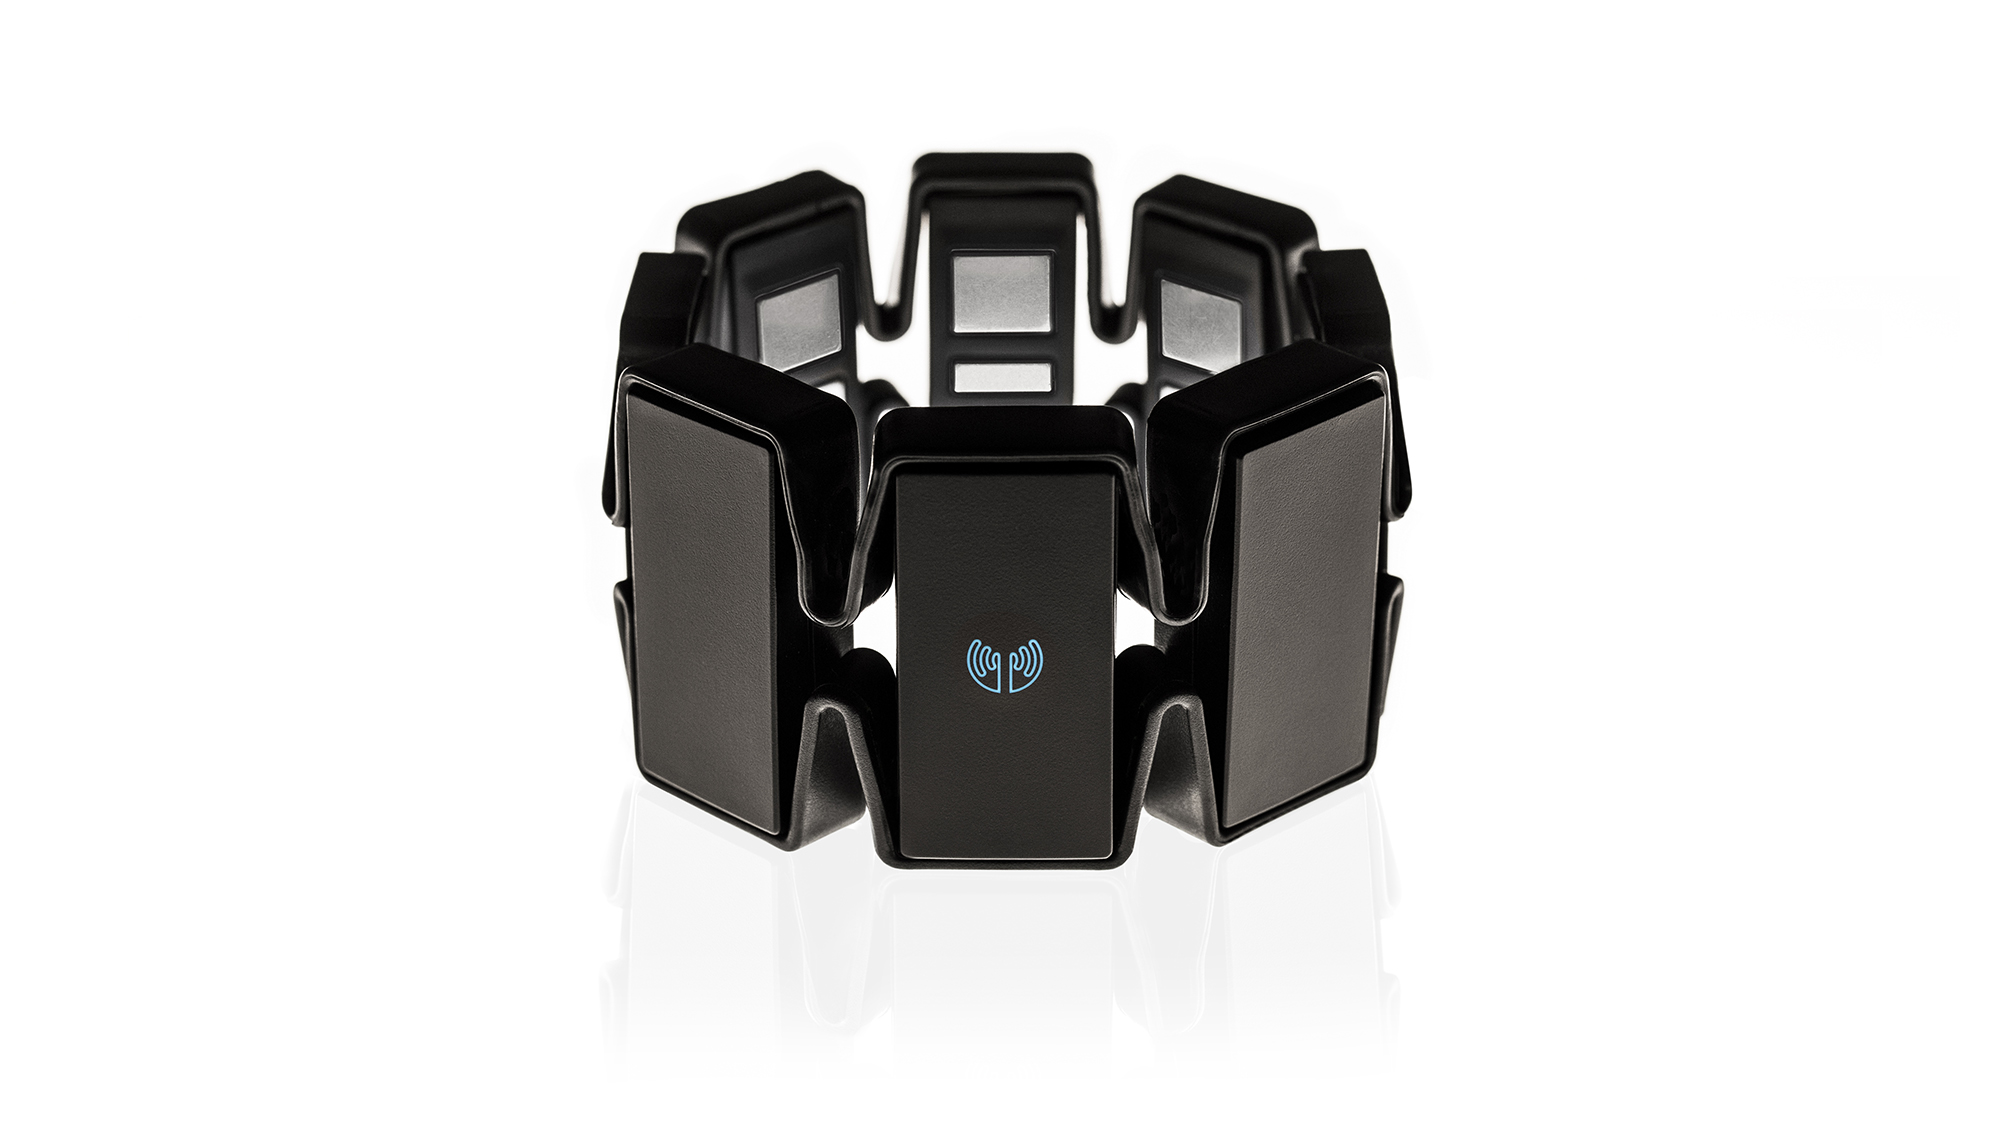
\includegraphics[width=11cm]{1388852727461}
  
Dato 15/6 - 2015 \newline

Ingeniørhøjskolen Aarhus Universitet \newline



\end{minipage}
\restoregeometry
\thispagestyle{empty}
\addtocontents{toc}{\protect\thispagestyle{empty}}
\tableofcontents*

%\newpage
% \thispagestyle{empty}
% \mbox{}
%\newpage
 

% Setup header and footer
\pagestyle{fancy}
\fancyhf{} % Clear all header an footer fields 
\renewcommand{\headrulewidth}{0pt} % Delete headruler
\fancyhead[R]{
\includegraphics[height=40pt]{header}} % Insert picture in left side of header
%\fancyhead[R]{\rightmark} % insert chapter title in right side of header
\fancyfoot[LE,RO]{\thepage} % insert pagenumber on right side of even page, left side of odd page 
%\setcounter{page}{1}

\chapter{Indledning}
\thispagestyle{fancy}
\chapter{Systembeskrivelse}
\label{chp:systembeskrivelse}
På baggrund af projektafgrænsningen vil dette kapitel præsenterere det system, som udgør rammerne for systemets udvikling. I figur \ref{fig:systembeskrivelse} forsøges det afgrænsede projekt beskrevet. Systemet beskrives som en mobilapplikation kørende på flere Windows Phone 8 enheder, en serverapplikation kørende på en Windows 7 eller nyere og en database, hvor relevante data opbevares. Det endelige system udvikles som et proof of concept til festivaller og navngives \textit{Mingle}.

\figur{systembeskrivelse.jpg}{Beskrivelse af systemet}{fig:systembeskrivelse}{1}

Det er målet igennem en mobilapplikation at støtte festivalgæsterne i socialisering og skabelse af nye venskaber. Dette gøres med et spørgsmålsspil, hvor to personer i samarbejde skal svare på spørgsmål om hinanden. Mobilapplikationen, serverapplikationen og databasen giver tilsammen denne personlige spiloplevelse.

For at skabe en personliggørelse af spillet er systemet tæt koblet med Facebook, hvorfra relevante informationer om brugerne hentes og gemmes i databasen. Når en bruger ønsker at logge ind benyttes email og adgangskode til Facebook. Hvis en bruger ønsker at benytte Mingle, er en Facebook bruger derfor et krav. 

Når et spørgsmålsspil startes fremvises det samme spørgsmål på mobilapplikationerne. Disse spørgsmål modtages fra serveren, som henter dem fra databasen. På databasen opbevares både spørgsmål og tilhørende svarmuligheder.

Ved et gennemført spil optjenes point. Disse point gemmes ligeledes i databasen og kan benyttes til at købe varer på festivaller. En festivalmedarbejder  verificerer købet, og pointene trækkes fra brugerens totale antal point.


Da Mingle har fokus på at skabe nye venskaber, sættes en begrænsning, hvor der udelukkende tildeles point for første spil som i samarbejde er vundet. Dette realiseres igennem en historik, som serveren håndterer og gemmer på databasen.






 

 
\chapter{Funktionelle krav} 
\label{chp:funktionellekrav}

\section{Indledning}
I dette kapitel indledes med en beskrivese af de funktionelle krav. Disse beskrives ved hjælp af use cases og indledes med et UML use case diagram, som hjælper læseren med at skabe overblik over de forskellige use cases, som herefter beskrives dybdegående

\section{Overblik over use cases}
I følgende beskrives de funktionelle krav igennem 7 forskellige  fully dressed use cases. 

Ved benævnelse af \emph{system} refereres der til \emph{mobilapplikationen}, \emph{serverapplikation} med dertilhørende \emph{database}.


\section{Aktørbeskrivelse}
Aktørerne som fremgår af use case diagrammet, og deres interaktion med systemet beskrives herefter.

\subsection{Bruger}
Bruger er den primære aktør i samtlige use cases. Det er brugeren der ønsker at benytte mobilapplikationen på sin mobile enhed. Brugeren ønsker at spille spørgsmålsspillet med andre festivalgæster, indtjene point i samarbejde med andre festivalgæster samt indløse point ved en festivalmedarbejder

\subsection{Festivalmedarbejder}
Festivalmedarbejder er en medarbejder på festivallen, som Bruger indløser sine point hos ved køb af en vare på festivallen.

\subsection{Facebook}
Facebook er et socialt netværk hvorfra oplysninger omkring brugere hentes. Et Facebook login er påkrævet for brugere af systemet, da der herfra indhentes de fornødne brugerinformationer.

\newpage

\section{Ordforklaringer}

\subsubsection{Mobilapplikationen:}
Refererer til den mobilapplikation, der kører på Brugers og Festivalgæsts enheder. Mobilapplikationen kommunikerer med resten af systemet

\subsubsection{Enhed:}
Refererer til en smartphone, som mobilapplikationen kører på.

\subsubsection{Spørgsmålspil:}
Refererer til det spil, som Bruger spiller med Festivalgæst gennem mobilapplikationerne på deres smartphones for at optjene point. Spillet består af en række spørgsmål, som både Bruger og Festivalgæst skal svare ens på.

\subsubsection{Point:}
Refererer til den digitale møntfod, som Bruger kan optjene ved at spille spørgsmålsspillet med nye festivalgæster. Møntfoden benyttes til at købe varer for hos Festivalmedarbejder.

\subsubsection{Unikt id:}
Refererer til det unikke id, som Bruger får tildelt ved første facebook login, og som derfra er Systems unikke reference til brugeren.

\subsubsection{Sammenkobling}
Refererer til at to brugere kobles sammen ved at udveksle deres unikke id'er. En sammenkobling opfattes for systemet som to unikke bruger-id'er og et tidsstempel samt en indikator for, om brugerne har modtaget point for sammenkoblingen.

\subsubsection{Historik}
Refererer til en oversigt over Brugers tidligere sammenkoblinger. Bruger kan derved se udvalgte facebookoplysninger på andre brugere, som Bruger tidligere har været i kontakt med via mobilapplikationen.

 \newpage


% Command \figur{filename}{caption}{label}{width} 
\figur{Krav/Kontekstdiagram.png}{Use Case Context Diagram:Use case 1-7}{Fig:UC: 1-7}{1}

\newpage

\section{UC1: Log ind}

\begin{tabular}{ >{\raggedleft} p{3cm} | p{12cm} }
Mål: & Bruger er logget ind. \\
Initiator: & Bruger \\
Primær aktør: & Bruger \\
Sekundær aktør: & Facebook \\
Forudsætning: & Mobilapplikationen er opstartet på Brugers enhed \newline
Dataforbindelse tilgængelig
 \\
 & \\
Hovedforløb:  & \begin{enumerate}[label=\arabic*.),itemjoin={\newline},topsep=0pt,partopsep=0pt,itemsep=0pt,leftmargin=*]   
\item Mobilapplikationen informerer om krav til forbindelse med Brugers Facebookprofil. \newline
[Extension 1: Bruger er allerede logget ind]
\item Bruger indtaster brugernavn og adgangskode til Facebook og bekræfter. \newline
[Extension 2: Bruger falsificerer]
\item System henter informationer fra Facebook samt det unikke id fra mobilapplikationen og fremviser hovedmenuen for Bruger.
\end{enumerate}\\
Extension 1: & [Bruger er allerede logget ind] \newline
\begin{enumerate}[label=\arabic*.),itemjoin={\newline},topsep=0pt,partopsep=0pt,itemsep=0pt,leftmargin=*]   
\item Use casen genoptages ved hovedforløb 3.) 
\end{enumerate} \\
Extension 2: & [Bruger falsificerer] \newline
\begin{enumerate}[label=\arabic*.),itemjoin={\newline},topsep=0pt,partopsep=0pt,itemsep=0pt,leftmargin=*]   
\item Use casen genoptages ved hovedforløb 2.)
\end{enumerate} \\
& \\
\end{tabular}


\newpage

\section{UC2: Forbind enheder}
\begin{tabular}{ >{\raggedleft} p{3cm} | p{12cm} }
Mål: & Brugers enhed er sammenkoblet med Festivalgæsts enhed. \\
Initiator: & Bruger \\
Primær aktør: & Bruger \\
Sekundær aktør: & Festivalgæst  \\
Reference: & UC3 \\
Forudsætning: & Bruger befinder sig i hovedmenuen
 \\
 & \\
Hovedforløb:  & \begin{enumerate}[label=\arabic*.),itemjoin={\newline},topsep=0pt,partopsep=0pt,itemsep=0pt,leftmargin=*]   
\item Bruger og Festivalgæst vælger at Mingle i hovedmenuen
\item Mobilapplikationen fremviser sammenkoblingsmenuen
\item Bruger vælger at oprette et spil
\item Mobilapplikationen fremviser Brugers id
\item Festivalgæst vælger at deltage i et spil
\item Mobilapplikationen fremviser muligheden for at indtaste id
\item Bruger udveksler unikt id med Festivalgæst. 
\item Festivalgæst indtaster Brugers id og accepterer. \newline
[Extension 1: Bruger og Festivalgæst har tidligere i samarbejde vundet spørgsmålsspillet]
[Extension 2: Bruger indtaster ikke korrekt id]
\item System forbinder Bruger med Festivalgæst og informerer herom.
\item Bruger og Festivalgæst accepterer. \newline
\item Use case 3 påbegyndes.
\end{enumerate}\\
Extension 1: & [Bruger og Festivalgæst har tidligere i samarbejde vundet spørgsmålsspillet]
\vspace{2 mm}
\begin{enumerate}[label=\arabic*.),itemjoin={\newline},topsep=0pt,partopsep=0pt,itemsep=0pt,leftmargin=*]   
\item System registrerer, at Bruger og Festivalgæst tidligere i samarbejde har vundet et spørgsmålsspil. Bruger og Festivalgæst informeres om at der således ikke optjenes point
\item Use casen genoptages ved hovedforløb 3.)
\end{enumerate} \\
Extension 2: & [Bruger indtaster ikke korrekt id]
\vspace{2 mm}
\begin{enumerate}[label=\arabic*.),itemjoin={\newline},topsep=0pt,partopsep=0pt,itemsep=0pt,leftmargin=*]   
\item System registrerer at ingen med det indtastede id ønsker at spille, og bruger informeres om fejlindtastelse.
\item Use casen genoptages ved hovedforløb 2.)
\end{enumerate} \\
& \\
& \\
\end{tabular}

\newpage

\section{UC3: Spil nyt spil}
\begin{tabular}{ >{\raggedleft} p{3cm} | p{12cm} }
Mål: & Bruger og Festivalgæst har gennemført spørgsmålsspil og modtaget point. \\
Initiator: & Startes af UC2 \\
Primær aktør: & Bruger \\
Sekundær aktør: & Festivalgæst  \\
Reference: & UC2: Enheder forbindes \\
Forudsætning: & Målet for UC2: Enheder forbindes er opnået
 \\
 & \\
Hovedforløb:  & \begin{enumerate}[label=\arabic*.),itemjoin={\newline},topsep=0pt,partopsep=0pt,itemsep=0pt,leftmargin=*]   
\item Brugers og Festivalgæsts mobilapplikationer fremviser spørgsmål og svarmuligheder.
\item Bruger og Festivalgæst vælger samme svar. \newline
[Extension 1: Bruger og Festivalgæst vælger ikke samme svar] \newline
[Extension 2: Bruger annullerer spørgsmålsspillet] \newline
[Extension 3: Festivalgæst annullerer spørgsmålspillet]
\item Mobilapplikationerne informerer Bruger og Festivalgæst om korrekt svar. Hovedforløb startes på ny fra 1.) til tre korrekte svar er opnået.
\item System tildeler point og informerer Bruger og Festivalgæst herom\newline 
[Extension 4: Bruger og Festivalgæst har tidligere i samarbejde vundet spørgsmålsspillet] 
\newline
\item Mobilapplikationerne gemmer sammenkobling mellem Festivalgæst og Bruger i historik og hovedmenuen fremvises mobilapplikationerne.
\end{enumerate}\\
Extension 1: &  [Bruger og Festivalgæst vælger ikke samme svar]
\vspace{2 mm}
\begin{enumerate}[label=\arabic*.),itemjoin={\newline},topsep=0pt,partopsep=0pt,itemsep=0pt,leftmargin=*]   
\item Mobilapplikationen informerer om at Bruger og Festivalgæst har svaret forkert.
\item Spørgsmålsspillet stoppes og Bruger og Festivalgæst informeres herom
\item Bruger og Festivalgæst accepterer.
\item Use case afsluttes og hovedmenuen fremvises
\end{enumerate} \\
Extension 2: &  [Bruger annullerer spørgsmålsspillet]
\vspace{2 mm}
\begin{enumerate}[label=\arabic*.),itemjoin={\newline},topsep=0pt,partopsep=0pt,itemsep=0pt,leftmargin=*]   
\item Mobilapplikationerne informerer Bruger og Festivalgæst om, at spørgsmålsspillet er annulleret.
\item Use case afsluttes og hovedmenuen fremvises
\end{enumerate} \\
\end{tabular}

\newpage

\begin{tabular}{ >{\raggedleft} p{3cm} | p{12cm} }
& \\
& \\
Extension 3: &  [Festivalgæst annullerer spørgsmålsspillet]
\vspace{2 mm}
\begin{enumerate}[label=\arabic*.),itemjoin={\newline},topsep=0pt,partopsep=0pt,itemsep=0pt,leftmargin=*]   
\item Mobilapplikationerne informerer Bruger og Festivalgæst om, at spørgsmålsspillet er annulleret.
\item Use case afsluttes og hovedmenuen fremvises
\end{enumerate} \\
Extension 4: & [Bruger og Festivalgæst har tidligere i samarbejde vundet spørgsmålsspillet]
\vspace{2 mm}
\begin{enumerate}[label=\arabic*.),itemjoin={\newline},topsep=0pt,partopsep=0pt,itemsep=0pt,leftmargin=*]   
\item System tildeler ikke point og informerer Bruger og Festivalgæst herom.
\item Bruger og Festivalgæst accepterer
\item Use casen genoptages ved hovedforløb 5.)
\end{enumerate} \\
\end{tabular}

\newpage

\section{UC4: Aflæs point}
\begin{tabular}{ >{\raggedleft} p{3cm} | p{12cm} }
Mål: & Bruger har aflæst point. \\
Initiator: & Mobilapplikationen \\
Primær aktør: & Bruger \\
Sekundær aktør: &  \\
Forudsætning: & Bruger befinder sig i hovedmenuen.
 \\
 & \\
Hovedforløb:  & \begin{enumerate}[label=\arabic*.),itemjoin={\newline},topsep=0pt,partopsep=0pt,itemsep=0pt,leftmargin=*]   
\item Mobilapplikationen fremviser antal optjente point i hovedmenuen.
\item Bruger aflæser antal optjente point.
\end{enumerate}\\
& \\
\end{tabular}



\section{UC5: Indløs point}
\begin{tabular}{ >{\raggedleft} p{3cm} | p{12cm} }
Mål: & Bruger har indløst point og modtaget vare. \\
Initiator: & Bruger \\
Primær aktør: & Bruger \\
Sekundær aktør: & Festivalmedarbejder  \\
Forudsætning: & Bruger befinder sig i hovedmenuen. \newline
Dataforbindelse tilgængelig.
 \\
 & \\
Hovedforløb:  & \begin{enumerate}[label=\arabic*.),itemjoin={\newline},topsep=0pt,partopsep=0pt,itemsep=0pt,leftmargin=*]   
\item Bruger vælger at indløse point.
\item Mobilapplikationen fremviser købsmenu.
\item Bruger vælger ønsket vare.  \newline
[Extension 1: Bruger har ikke nødvendigt antal point] 
\item Mobilapplikationen fremviser verificering, og informerer Bruger om at overrække enheden til Festivalmedarbejder.
\item Bruger giver enhed til Festivalmedarbejder.
\item Festivalmedarbejder verificerer købet i mobilapplikationen.
\item Mobilapplikationen fjerner point tilsvarende købets værdi fra Bruger og 
fremviser hovedmenuen.

\end{enumerate}\\
Extension 1: & [Bruger har ikke nødvendigt antal point]
\vspace{2 mm}
\begin{enumerate}[label=\arabic*.),itemjoin={\newline},topsep=0pt,partopsep=0pt,itemsep=0pt,leftmargin=*]   
\item Applikation informerer Bruger om, at der ikke er optjent tilstrækkeligt antal point til at indløse ønskede vare.
\item Bruger accepterer.
\item Use case genoptages fra hovedforløb 2.)
\end{enumerate} \\
& \\
\end{tabular}

\newpage 

\section{UC6: Aflæs historik}
\begin{tabular}{ >{\raggedleft} p{3cm} | p{12cm} }
Mål: & Bruger har aflæst historik over sammenkoblinger og er tilbage i hovedmenuen. \\
Initiator: & Bruger \\
Primær aktør: & Bruger \\
Sekundær aktør: &  Facebook \\
Forudsætning: & Bruger befinder sig i hovedmenuen
 \\
 & \\
Hovedforløb:  & \begin{enumerate}[label=\arabic*.),itemjoin={\newline},topsep=0pt,partopsep=0pt,itemsep=0pt,leftmargin=*]   
\item Bruger vælger historik i hovedmenuen.
\item Mobilapplikationen fremviser historik over sammenkoblinger og dertilhørende Facebookoplysninger.  \newline
[Extension 1: Bruger har ikke haft nogen sammenkoblinger]
\item Bruger aflæser historik og trykker sig tilbage til hovedmenuen.
\item Mobilapplikationen fremviser hovedmenuen.
\end{enumerate}\\
Extension 1: & [Bruger har ikke haft nogen sammenkoblinger]
\vspace{2 mm}
\begin{enumerate}[label=\arabic*.),itemjoin={\newline},topsep=0pt,partopsep=0pt,itemsep=0pt,leftmargin=*]   
\item Mobilapplikationen informerer Bruger om, at der endnu ikke er forekommet nogen sammenkoblinger og opfordrer Bruger til at søge nye venskaber.
\item Bruger trykker sig tilbage til hovedmenuen.
\item Applikationen fremviser hovedmenuen.
\end{enumerate} \\
& \\
\end{tabular}


\section{UC7: Log ud}
\begin{tabular}{ >{\raggedleft} p{3cm} | p{12cm} }
Mål: &  Bruger er logget ud \\
Initiator: & Bruger \\
Primær aktør: & Bruger \\
Sekundær aktør: &  Facebook\\
Forudsætning: & Bruger befinder sig i hovedmenuen i mobilapplikationen.
 \\
 & \\
Hovedforløb:  & \begin{enumerate}[label=\arabic*.),itemjoin={\newline},topsep=0pt,partopsep=0pt,itemsep=0pt,leftmargin=*]   
\item Bruger vælger at logge ud i hovedmenuen.
\item Mobilapplikationen logger Bruger ud, og UC1 hovedforløb 1.) påbegyndes.
\end{enumerate}\\
& \\
\end{tabular}




\chapter{Ikke funktionelle krav} 
\label{chp:IkkeFunktionelleKrav}

\section{Indledning}
I dette kapitel beskrives projektets ikke funktionelle krav.


\section{Platform}
\begin{itemize}
\item Applikationen udvikles til:
\begin{itemize}
\item Windows Phone 8 og nyere
\end{itemize} 

\end{itemize}



\bibliographystyle{plainnat}
\bibliography{bibliografi}% Selects .bib file AND prints bibliography
\thispagestyle{fancy}

%\listoftodos % Make a list of todo's
\end{document}